\documentclass[tikz, border=10pt]{standalone}
\usepackage[utf8]{inputenc}
\usetikzlibrary{shapes.geometric, arrows.meta, positioning, fit, backgrounds, calc}

\begin{document}
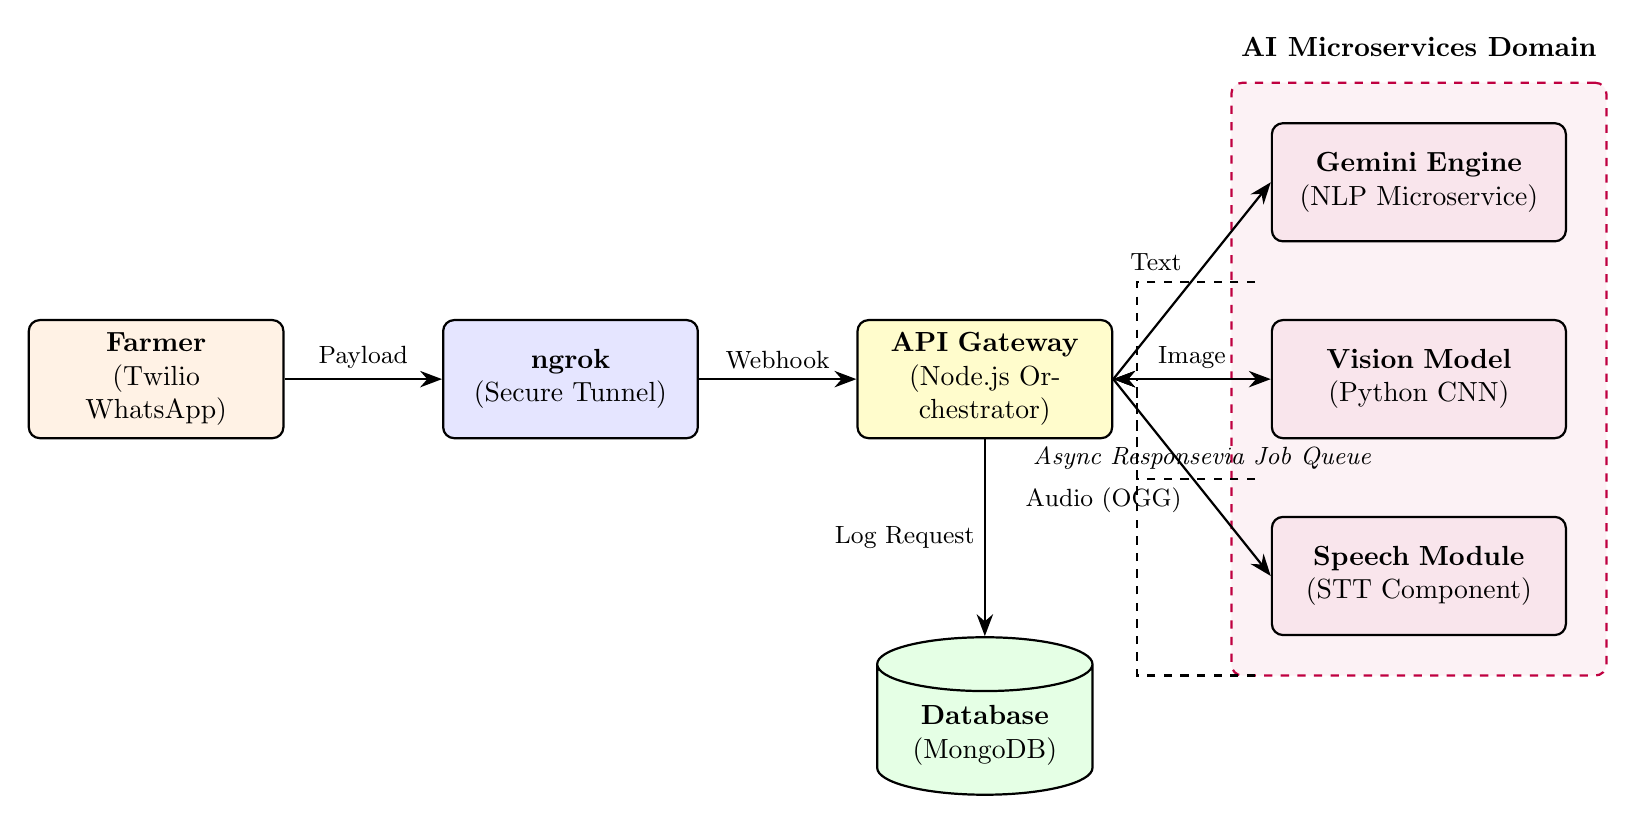
\begin{tikzpicture}[
    node distance=1.5cm and 2cm,
    box/.style={rectangle, draw=black, thick, fill=blue!10, text width=3cm, align=center, minimum height=1.5cm, rounded corners},
    db/.style={cylinder, draw=black, thick, fill=green!10, shape border rotate=90, aspect=0.25, text width=2.5cm, align=center, minimum height=2cm},
    micro/.style={rectangle, draw=black, thick, fill=purple!10, text width=3.5cm, align=center, minimum height=1.5cm, rounded corners},
    arrow/.style={-{Stealth[scale=1.2]}, thick}
]

    % Nodes
    \node[box, fill=orange!10] (farmer) {\textbf{Farmer} \\ (Twilio WhatsApp)};
    \node[box, right=of farmer] (ngrok) {\textbf{ngrok} \\ (Secure Tunnel)};
    \node[box, right=of ngrok, fill=yellow!20] (api) {\textbf{API Gateway} \\ (Node.js Orchestrator)};
    
    \node[db, below=of api, yshift=-1cm] (mongo) {\textbf{Database} \\ (MongoDB)};
    
    \node[micro, right=of api, yshift=2.5cm] (gemini) {\textbf{Gemini Engine} \\ (NLP Microservice)};
    \node[micro, right=of api, yshift=0cm] (vision) {\textbf{Vision Model} \\ (Python CNN)};
    \node[micro, right=of api, yshift=-2.5cm] (speech) {\textbf{Speech Module} \\ (STT Component)};

    % Background bounding box for AI Microservices
    \begin{scope}[on background layer]
        \node[draw=purple, thick, dashed, fill=purple!5, fit=(gemini) (vision) (speech), inner sep=0.5cm, rounded corners, label={[anchor=south, yshift=0.2cm, font=\bfseries]above:AI Microservices Domain}] (ai_domain) {};
    \end{scope}

    % Arrows
    \draw[arrow] (farmer) -- node[above, font=\small] {Payload} (ngrok);
    \draw[arrow] (ngrok) -- node[above, font=\small] {Webhook} (api);
    
    \draw[arrow] (api) -- node[left, font=\small] {Log Request} (mongo);
    
    \draw[arrow] (api.east) -- node[above left, font=\small] {Text} (gemini.west);
    \draw[arrow] (api.east) -- node[above, font=\small] {Image} (vision.west);
    \draw[arrow] (api.east) -- node[below left, font=\small] {Audio (OGG)} (speech.west);
    
    \draw[arrow, dashed] (gemini.south west) ++(-0.2,-0.5) -- ++(-1.5,0) |- (api.east);
    \draw[arrow, dashed] (vision.south west) ++(-0.2,-0.5) -- ++(-1.5,0) |- (api.east);
    \draw[arrow, dashed] (speech.south west) ++(-0.2,-0.5) -- ++(-1.5,0) |- (api.east);
    
    \node at ($(api)!0.5!(vision)$) [yshift=-1cm, font=\small\itshape] {Async Response\\via Job Queue};

\end{tikzpicture}
\end{document}
